\documentclass[usepdftitle=false,unknownkeysallowed,8pt]{beamer}
\usetheme{egupico} % beamerthemeegupico.sty
% change some colors:
\definecolor{bgcolor}            {rgb}{0.83, 0.88, 0.85}
\definecolor{buttonpassivecolor} {rgb}{0,0.6274,0.8353} 
\definecolor{buttonactivecolor}  {rgb}{0,0.4,0.4}


\usepackage[english]{babel} % English language/hyphenation


% Set title and Author informations here
\def\shortauthor{A. K\"ohler \& R. Sander}
\def\shorttitle{PICO \LaTeX}

\title{beamer theme \textit{egupico}: A \LaTeX template for copernicus conference PICO presentations}

\author{Anselm K\"ohler \& Rolf Sander}

\institute{Git Repository: \url{https://github.com/snowtechblog/pico-latex-presentation}}

\newcommand{\myhrule}{\mbox{}\hrulefill\\[7mm]}



\begin{document}

%%%%%%%%%%%%%%%%%%%%%%%%%%%%%%%%%%%%%%%%%%%%%%%%%%%%%%%%%%%%%%%%%%%%%%%%%%%%%%

\picosection{home}{HOME}{}
\begin{frame}

  \begin{center}
    \centering \usebeamerfont{title} \inserttitle\\\medskip
    \centering \usebeamerfont{author} \insertauthor\\\medskip
    \centering \usebeamerfont{institute} \insertinstitute
  \end{center}
  \vspace{3cm}
  \begin{columns}%[t]
    \begin{column}{0.66\textwidth}
      \large PICO: presenting interactive content -- \\ a crossbreed between talk and poster
    \end{column}
    \begin{column}{0.3\textwidth}
      \fbox{\includegraphics[width=\columnwidth]{figures/graphic_EGU_PICO_logo}}
    \end{column}
  \end{columns}

\end{frame}

%%%%%%%%%%%%%%%%%%%%%%%%%%%%%%%%%%%%%%%%%%%%%%%%%%%%%%%%%%%%%%%%%%%%%%%%%%%%%%

 \picosection{howto}{How to}{How to use \& how to change appearance}
 \begin{frame}

   Main thing about PICO is that you use a touchscreen to navigate through your presentation. Therefore, the \textit{egupico} beamer theme generates automatically a navigation bar at the bottom of the page.

   \begin{itemize}%
   \item Best to have for every new beamer frame an own navigation button, otherwise the presentation becomes very messy and hard to navigate through.
   \item So, a usual call for any new frame should follow each time the new command \texttt{\textbackslash picosection} for a new navigation button
   \item command: \texttt{\textbackslash picosection} has three inputs: internal name of section (NO spaces!), navigation button text (should be short), and section / frame title\\
    \fbox{\includegraphics[width=0.6\columnwidth]{figures/picosection}}
  \item if you want some traditional navigation buttons like forward/backward etc. you can edit the style sheet \texttt{beamerthemeegupico.sty} below line 101.

   \end{itemize}

   %\lstinline!\picosection!
   %(\lstinline!\begin{frame}...!) 


 \end{frame}

%%%%%%%%%%%%%%%%%%%%%%%%%%%%%%%%%%%%%%%%%%%%%%%%%%%%%%%%%%%%%%%%%%%%%%%%%%%%%%

\picosection{usability}{IMPORTANT}{Important note for your successful presentation}
\begin{frame}

  IMPORTANT NOTE:

  In the last years, there are many complains about the PICO sessions, partly because of the "random" page flips. The PICO touchscreens are usually to sensitive and it is very difficult to explain people your presentation, when even a 2cm distance of the finger to the screen flips the page... You want to disable the Acrobat PDF reader default fullscreen setting every time you open your presentation! 

\vspace{0.5cm}

\fbox{\includegraphics[width=0.8\columnwidth]{figures/acrobat-settings}}

\begin{itemize}
  \item to open preferences menu on PICO-screen, click on the cc-logo: 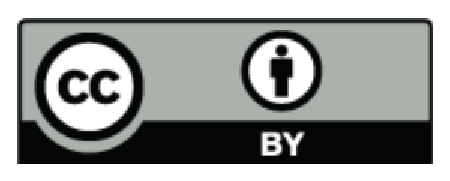
\includegraphics[height=0.04\textheight]{figures/CreativeCommons_Attribution_License} in the bottom right. It is linked against the Acrobat-Settings (Nothing will open if you use a different PDF viewer.)
  \item disable the option: "left click to go forward one page ..."
\end{itemize}


\end{frame}

%%%%%%%%%%%%%%%%%%%%%%%%%%%%%%%%%%%%%%%%%%%%%%%%%%%%%%%%%%%%%%%%%%%%%%%%%%%%%%

\picosection{otherchanges}{Other changes}{Other changes}
\begin{frame}
  
      \begin{itemize}
        \item in the beginning of the latex file, there are colors defined. you can change as you want. other changes are free to you. Implement what you want...

        \item read the documentation of beamer class to find out more about style options you have: \url{https://ctan.org/pkg/beamer?lang=en}

        \item please advance the GIT repository with your changes!
        \item if you want to tell us something: \url{anselm.koehler@gmail.com} or
        \url{rolf.sander@mpic.de}
      \end{itemize}
      
\end{frame}

%%%%%%%%%%%%%%%%%%%%%%%%%%%%%%%%%%%%%%%%%%%%%%%%%%%%%%%%%%%%%%%%%%%%%%%%%%%%%%

\picosection{todo}{TODO}{TODO and how to improve the template}
\begin{frame}
  
      \begin{itemize}
        \item to generate the navigation bar, the template produces two \texttt{.tex} files. this works, but is not the nicest solution. (in case you have compiling issues, remove these additional helper files and rebuild.)
      \end{itemize}
      
\end{frame}

\end{document}

%%%%%%%%%%%%%%%%%%%%%%%%%%%%%%%%%%%%%%%%%%%%%%%%%%%%%%%%%%%%%%%%%%%%%%%%%%%%%% 
